%----------------------------------------------------------------------------
\chapter{\bevezetes}

A modern tudomány egyik legnagyobb kihívása a komplex biológiai rendszerek dinamikájának megértése és előrejelzése. Az ökoszisztémák vizsgálata a valóságban gyakran akadályokba ütközik: a folyamatok időigényesek, a beavatkozások pedig visszafordíthatatlanok vagy etikailag megkérdőjelezhetőek lehetnek. A számítógépes szimulációk ezzel szemben biztonságos, költséghatékony és reprodukálható környezetet biztosítanak a populációgenetikai és ökológiai elméletek teszteléséhez.

A diplomamunka alapvető motivációja egy olyan digitális laboratórium létrehozása volt, amely képes vizuálisan és adat szintjén is reprezentálni a természetes szelekciót és a fajok közötti interakciókat. A projekt célja nem csupán egy látványos vizualizáció elkészítése, hanem egy olyan robusztus szoftverarchitektúra kialakítása, amely alkalmas lehet tudományos igényű adatgyűjtésre és elemzésre.

A projektem gyökerei a BSc képzés idejére nyúlnak vissza, ahol az első ágensalapú modellek implementálása megtörtént. A koncepció kidolgozásakor inspirációként szolgált Sebastian Lague ismert ökoszisztéma-szimulációs projektje, amely rávilágított a Unity3D motorban rejlő lehetőségekre a biológiai modellezés terén.

Az ötletet a klasszikus evolúcióelmélet adta, amelynek egyik legismertebb gyakorlati példája a darwini pintyek csőrmorfológiájának adaptációja a környezeti táplálékforrásokhoz (lásd az \ref{fig:darwin_finches}. ábrát). Elsősorban fizikai és morfológiai jegyek változásán keresztül mutatja be a természetes szelekciót, a jelen diplomamunka egy ettől eltérő, ám valamilyen módon mégis analóg megközelítést alkalmaz. 
A koncepció elméleti hátterét és a természetes szelekció modellekben betöltött szerepét Purdom is részletesen tárgyalja \cite{Georgia14}.

\begin{figure}[h!]
\centering
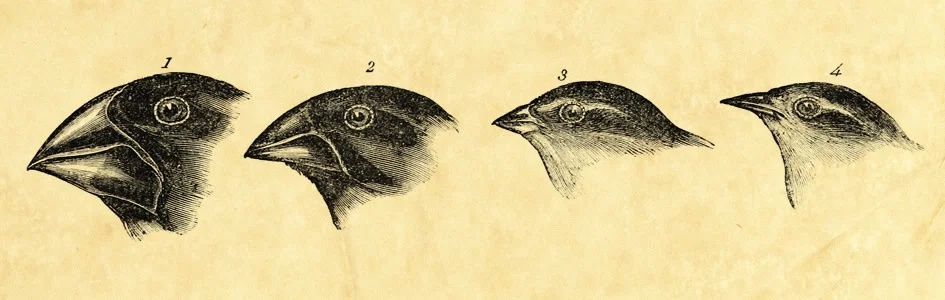
\includegraphics[width=0.7\textwidth]{figures/evolution.png}
\caption{A darwini pintyek adaptív radiációja: a csőr alakjának változása a táplálkozási specializáció függvényében \cite{Georgia14}}
\label{fig:darwin_finches}
\end{figure}

A digitális laboratóriumomban a szelekciós nyomást nem a táplálék fizikai jellege, hanem a ragadozó-préda dinamika, közelebbről a rókák (\textit{Vulpes vulpes}) populációba történő bevezetése jelentette. A szimuláció során a morfológiai átalakulások helyett a viselkedési és fiziológiai tulajdonságok, mint például az ágensek futási sebessége vagy a kockázatvállalási hajlandóságot meghatározó bátorság, transzgenerációs eltolódásait vizsgáltam. A lassú egyedek eliminációja révén a rendszerben egy diszkrét, számszerűsíthető evolúciós nyomás alakult ki, amely kiváló alapot biztosított a későbbi statisztikai elemzésekhez és a komplex döntési folyamatok implementálásához.

Míg a kezdeti inspiráció a vizuális reprezentációra és az alapvető túlélési logikára fókuszált, a saját fejlesztésem hamar túllépett ezen a kereten. Az eddigi megoldásokhoz képest a hangsúly eltolódott a szoftvertechnológiai precizitás, a skálázhatóság és a professzionális adatkezelés irányába. A korábbi monolitikus struktúrát felváltotta egy moduláris felépítés, amely lehetővé tette a komplexebb, fajspecifikus viselkedésformák és az eseményvezérelt működés integrálását.

A dolgozatban bemutatott rendszer egy Unity3D alapú, eseményvezérelt ökoszisztéma-szimuláció. A keretrendszer legfőbb újdonsága a populációgenetikai folyamatok mély integrációja: az egyedek DNS-alapú öröklődési mechanizmusokkal rendelkeznek, amelyek meghatározzák fizikai jellemzőiket és viselkedési stratégiáikat.

A szimuláció során keletkező hatalmas mennyiségű adat hatékony kezelésére és valós idejű monitorozására egy InfluxDB adatbázisra épülő naplózó rendszert fejlesztettem ki. Az események továbbítása HTTP-alapú API hívásokon keresztül történik, az adatok vizuális megjelenítését és elemzését pedig egy Grafana dashboard biztosítja. Ez a felépítés lehetővé teszi, hogy a populációk változásait, a mutációk hatásait és a ragadozó-préda dinamikát ne csak a Unity környezetben, hanem külső statisztikai eszközökkel validált, interaktív grafikonok formájában is elemezhessük.

A dolgozat szerkezete a következőképpen alakul: A \textbf{\ref{chap:specifikacio}. fejezet} a feladatkiírás részletes elemzésével, a funkcionális és nem-funkcionális követelmények specifikációjával, valamint a felhasznált technológiák (különösen a Unity, az InfluxDB és a Grafana) bemutatásával foglalkozik. Az elméleti hátteret, az ökológiai alapmodelleket és a rokon szoftveres megoldásokat – kiemelve Sebastian Lague szimulációs munkásságát – a \textbf{\ref{chap:irodalom}. fejezet} részletezi. A \textbf{\ref{chap:architektura}. fejezet} tárgyalja a szimulációs rendszer teljes szoftverarchitektúráját, az eseményvezérelt modellt, a populációgenetikai logikát, valamint a három integrált döntési mechanizmus (FSM, Utility AI, FCM) tervezését és implementációját. Az elért mérési eredmények kritikai reflexióját, a teljesítményelemzést és a döntési modellek kísérleti összehasonlítását az \textbf{\ref{chap:ertekeles}. fejezet} tartalmazza, egyúttal kijelölve a jövőbeli fejlesztési irányokat. Végezetül a \textbf{\ref{chap:osszefoglalas}. fejezet} röviden összefoglalja a kutató-fejlesztő munka főbb konklúzióit.